\begin{figure*}[!t] \centerline{\includegraphics[width=\textwidth,page=2]{../figures/main_figures_draft.pdf}} \caption{\textbf{Thermodynamic sources.} (\textbf{A}) Provenance of every pK$_\mathrm{a}$ ladder shipped in the database, across all 45,708 compounds and 56,002 reactions. ChemAxon Marvin supplies 79.4\% of compounds and 81.6\% of reactions. \emph{Hatching} marks the share reached through a second route: the command-line calculator refuses polymers and organometallics as query molecules, so those are computed from SMILES through the Java plugin instead --- the same engine entered differently, agreeing to a median $|\Delta|$ of $0.0000$ over 300 compounds both routes accept. \emph{No ionizable site} is a result and not a gap --- Marvin reported no dissociable proton between pH $-2$ and $16$ for 1,242 compounds. The remainder carry no structure to compute from, which is a curation gap rather than a protonation one. (\textbf{B}) Reactions carrying a real energy from each source. (\textbf{C}) Reported uncertainty in kcal\,mol$^{-1}$, one axis per source because the three differ by more than an order of magnitude. The shaded band spans the 5th to 95th percentile, which is used in our classification scheme.} \label{fig:thermo} \end{figure*}

\subsection{Thermodynamics}\label{sec:results-thermo}

%% Counts measured 2026-09-08 from Biochemistry/reaction_*.json after the
%% Marvin 26.1 rebuild. Placeholders excluded per source: group contribution
%% dg = 1e7 (26,555 records); eQuilibrator sigma >= 2500 kcal/mol (3,386),
%% which is that source's refusal marker rather than an error bar.
The three predictors cover comparable fractions of the database and disagree substantially about how well they do it (Figure~\ref{fig:thermo}B). Uncertainty is reported on scales differing by more than an order of magnitude (Figure~\ref{fig:thermo}C): median 0.63\,kcal\,mol$^{-1}$ for eQuilibrator against 10.41 for group contribution and 17.01 for dGPredictor. 

\paragraph{Calibrating the reported errors against measurement.} That a source understates its error is measurable rather than asserted, and the experimental anchors are what measure it. For each source we collect one held-out prediction per anchored reaction --- a predicted energy and the uncertainty that source would report for it --- and divide the residual against the measured \drGo{} by that uncertainty. Measured this way, eQuilibrator's ratio has a root mean square of 8.06 and a median of 2.27, with only 28.7\% of reactions inside one standard deviation and 46.3\% inside two, indicating that eQuilibrator understates their error. Group contribution runs the other way, 73.6\% inside one standard deviation and a median ratio of 0.32 and dGPredictor is the best scaled of the three at 1.15 root mean square and 87.9\% inside one standard deviation. A researcher choosing by smallest reported error would systematically choose the source that understates it, which is the argument against promoting any single source. The grading in the next section calibrates each source's confidence against measurement rather than taking its uncertainty at face value.
